% !TeX program = xelatex
% !TeX encoding = UTF-8

\documentclass[12pt,a4paper]{article}

\usepackage{fontspec}
\defaultfontfeatures{Ligatures=TeX}
\IfFontExistsTF{TeX Gyre Termes}
  {\setmainfont{TeX Gyre Termes}}
  {\setmainfont{Latin Modern Roman}}
\setmonofont{Latin Modern Mono}[Scale=MatchLowercase]

\usepackage{amsmath,amssymb}
\usepackage{unicode-math}
\setmathfont{Latin Modern Math}
\usepackage[top=2cm,bottom=2cm,left=2.3cm,right=2.2cm]{geometry}
\usepackage[table]{xcolor}
\usepackage{array,booktabs,tabularx}
\usepackage{titlesec,fancyhdr}
\usepackage{graphicx}
\usepackage{float}
\usepackage{caption}
\usepackage{enumitem}
\usepackage{listings}
\usepackage{hyperref,bookmark}

\definecolor{TableHead}{HTML}{E8EDF2}
\definecolor{LinkBlue}{HTML}{1F4770}
\hypersetup{
  unicode=true,
  colorlinks=true,
  linkcolor=black,
  citecolor=black,
  urlcolor=LinkBlue,
  pdftitle={Kiểm định trung bình một mẫu - GPU}
}

\setlength{\parindent}{0pt}
\setlength{\parskip}{5pt}
\linespread{1.07}

\titleformat{\section}{\large\bfseries}{\thesection}{0.6em}{}
\titleformat{\subsection}{\normalsize\bfseries}{\thesubsection}{0.6em}{}
\titleformat{\subsubsection}{\normalsize\bfseries}{\thesubsubsection}{0.6em}{}
\titlespacing*{\section}{0pt}{11pt}{5pt}
\titlespacing*{\subsection}{0pt}{9pt}{4pt}
\titlespacing*{\subsubsection}{0pt}{7pt}{3pt}

\providecommand{\tightlist}{\setlength{\itemsep}{0pt}\setlength{\parskip}{0pt}}

\pagestyle{fancy}
\fancyhf{}
\fancyfoot[C]{\small Trang~\thepage}
\renewcommand{\headrulewidth}{0pt}

\lstset{
  basicstyle=\footnotesize\ttfamily,
  keywordstyle=\color{blue},
  commentstyle=\color{green!60!black},
  stringstyle=\color{red},
  showstringspaces=false,
  breaklines=true,
  numbers=left,
  numberstyle=\tiny\color{black},
  numbersep=5pt,
  tabsize=2,
  language=Python,
  xleftmargin=11pt,
  xrightmargin=11pt,
  frame=single
}
\AtBeginDocument{
  \renewcommand{\tablename}{Bảng}
  \renewcommand{\figurename}{Hình}
}

\begin{document}

\section{Thống kê suy diễn}

\subsection{Bài toán kiểm định trung bình một mẫu}

\subsubsection{Đề xuất phương pháp}

Theo chuẩn kỹ thuật phần cứng máy tính, khe cắm mở rộng PCIe~x16 trên bo mạch chủ cung cấp công suất tối đa $75$\,W; các card đồ họa vượt ngưỡng này bắt buộc phải sử dụng thêm đầu cấp nguồn phụ từ bộ nguồn (PSU)[cite: 6]. Do đó, việc kiểm định mức công suất thiết kế trung bình của thị trường GPU rời so với ngưỡng $75$\,W giúp đánh giá xu hướng thiết kế hệ thống cấp điện của phần cứng đồ họa.

\textbf{Bài toán.} Với mức ý nghĩa $\alpha = 0{,}05$ (độ tin cậy $95\%$), công suất thiết kế tối đa trung bình (\texttt{max\_power\_w}) của GPU rời có lớn hơn ngưỡng $75$\,W của khe PCIe hay không?

Bài toán sử dụng toàn bộ $n = 2\,057$ GPU rời trong tập dữ liệu sạch (\texttt{gpus\_analysis.parquet})[cite: 6]. Từ các đặc trưng thống kê mẫu, ta có trung bình mẫu $\bar{x} = 124{,}93$\,W, độ lệch chuẩn mẫu $s = 76{,}94$\,W, trung vị $120{,}00$\,W, $\text{IQR} = 107{,}00$\,W và sai số chuẩn của trung bình mẫu là:
\[
  SE = \frac{s}{\sqrt{n}} = \frac{76{,}94}{\sqrt{2\,057}} = 1{,}70\text{\,W}.
\]

Gọi $\mu$ là công suất thiết kế tối đa trung bình tổng thể của GPU rời. Cặp giả thuyết kiểm định một phía bên phải được thiết lập như sau:
\[
  H_0: \mu = 75\text{\,W}, \qquad H_1: \mu > 75\text{\,W}.
\]

\subsubsection{Phân tích kiểm định một mẫu}

\paragraph{Kiểm tra điều kiện phân phối chuẩn.}
Đặt $H_0$: dữ liệu \texttt{max\_power\_w} tuân theo phân phối chuẩn; $H_1$: không tuân theo phân phối chuẩn. Kiểm định Shapiro--Wilk cho giá trị $W = 0{,}954$ với $p = 6{,}16 \cdot 10^{-25} < 0{,}001$, bác bỏ giả thuyết phân phối chuẩn. Trên đồ thị Q--Q chuẩn (Hình~\ref{fig:one_sample_qq}), các điểm quan trắc ở vùng trung tâm bám khá sát đường tham chiếu đỏ nhưng cong lệch lên trên ở hai đầu mút, phản ánh phân bố dữ liệu bị lệch phải.

\begin{figure}[H]
  \centering
  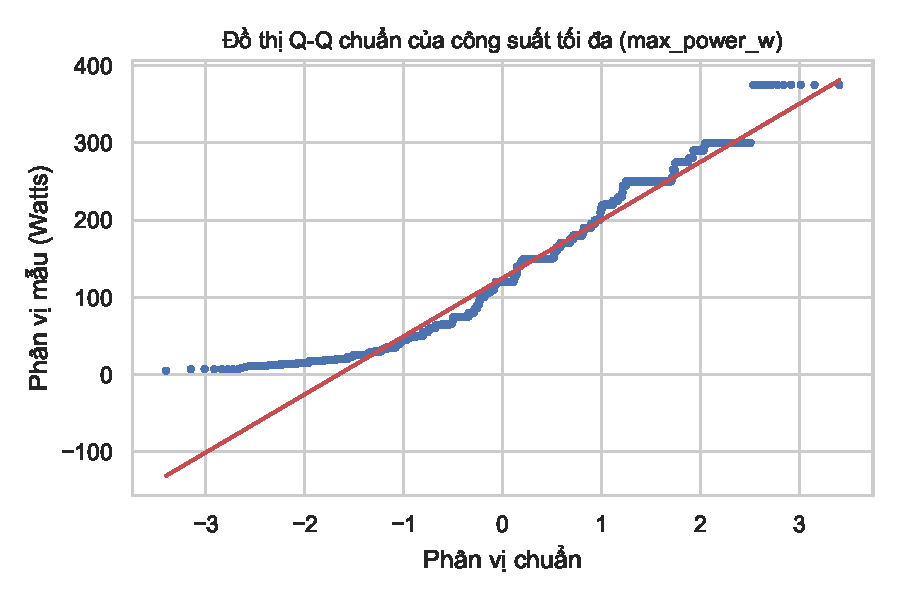
\includegraphics[width=0.64\linewidth]{one_sample_qq.pdf}
  \caption{Đồ thị Q--Q chuẩn của biến công suất tối đa \texttt{max\_power\_w} ($n = 2\,057$).}
  \label{fig:one_sample_qq}
\end{figure}

Tuy nhiên, vì cỡ mẫu rất lớn ($n = 2\,057 \gg 30$), theo Định lý giới hạn trung tâm (CLT)[cite: 7, 16], phân phối của trung bình mẫu $\bar{x}$ vẫn xấp xỉ phân phối chuẩn nên \textbf{kiểm định $t$ một mẫu} hoàn toàn hợp lệ.

\paragraph{Thực hiện kiểm định $t$ một mẫu và ước lượng khoảng tin cậy.}
Thống kê kiểm định $t$ với bậc tự do $\nu = n - 1 = 2\,056$ được tính bằng:
\[
  t_{qs} = \frac{\bar{x} - \mu_0}{SE} = \frac{124{,}93 - 75}{1{,}70} = 29{,}43.
\]
Với mức ý nghĩa $\alpha = 0{,}05$ (một phía phải), giá trị tới hạn là $t_{0{,}95;\ 2\,056} = 1{,}65$, suy ra miền bác bỏ là $RR = (1{,}65;\ +\infty)$. Giá trị quan sát $t_{qs} = 29{,}43$ nằm sâu trong miền bác bỏ với $p = 1{,}71 \cdot 10^{-159} < 0{,}001$, do đó ta bác bỏ giả thuyết $H_0$.

Đồng thời, khoảng tin cậy $95\%$ (hai phía) cho công suất thiết kế tối đa trung bình $\mu$ là:
\[
  CI_{95\%}(\mu) = \bar{x} \pm t_{0{,}975;\ 2\,056} \cdot SE = 124{,}93 \pm 1{,}96 \times 1{,}70 = [121{,}61;\ 128{,}26]\text{\,W}.
\]

\paragraph{Kiểm tra độ bền vững của kết quả.}
Do phân bố của biến \texttt{max\_power\_w} bị lệch phải bởi các dòng card đồ họa cao cấp có mức tiêu thụ lớn (lên tới $375$\,W), nhóm thực hiện thêm hai phép kiểm tra bổ trợ (tổng hợp ở Bảng~\ref{tab:one_sample_summary}) để bảo đảm kết luận không bị chi phối bởi giá trị ngoại lệ hay giả định phân phối chuẩn:
\begin{itemize}\tightlist
  \item \textbf{Kiểm định phi tham số Wilcoxon có dấu :} Phương pháp này kiểm định dựa trên thứ hạng và mức trung vị ($120{,}00$\,W) thay vì trung bình cộng, không yêu cầu giả định phân phối chuẩn và ít chịu ảnh hưởng bởi các điểm ngoại lệ. Với cặp giả thuyết một phía phải so với ngưỡng $75$\,W, kiểm định cho thống kê $W = 1\,553\,910$ và $p = 1{,}60 \cdot 10^{-134} < 0{,}001$, tiếp tục bác bỏ $H_0$.
  \item \textbf{Kiểm định $t$ trên thang đo logarit ($\ln P$):} Việc biến đổi dữ liệu sang thang logarit tự nhiên $\ln(\texttt{max\_power\_w})$ giúp giảm độ lệch phải và đưa phân bố về gần dạng đối xứng hơn. Kiểm định $t$ một mẫu so sánh trung bình của $\ln(\texttt{max\_power\_w})$ với $\ln(75)$ cho $t_{qs} = 15{,}02$ ($\nu = 2\,056$, $p = 8{,}98 \cdot 10^{-49} < 0{,}001$). Khi biến đổi ngược bằng hàm mũ ($e^{\overline{\ln P}}$), trung bình nhân của công suất GPU rời đạt $97{,}34$\,W (khoảng tin cậy $95\%$: $[94{,}08;\ 100{,}71]$\,W), vẫn cao hơn rõ rệt so với mức $75$\,W.
\end{itemize}

\begin{lstlisting}[language=Python]
import numpy as np
import pandas as pd
from scipy import stats

# Doc du lieu va tinh cac dai luong mau
df = pd.read_parquet("data/processed/gpus_analysis.parquet")
power = df["max_power_w"].dropna().astype(float)
n = len(power)
mean_val, sd_val = power.mean(), power.std(ddof=1)
se_val = sd_val / np.sqrt(n)
mu_0 = 75.0

# 1. Kiem tra tinh chuan Shapiro-Wilk
stats.shapiro(power)

# 2. Kiem dinh t mot mau (H1: mu > 75) va KTC 95%
t_stat, p_two = stats.ttest_1samp(power, popmean=mu_0)
p_right = p_two / 2
t_crit = stats.t.ppf(0.975, df=n - 1)
ci_95 = (mean_val - t_crit * se_val, mean_val + t_crit * se_val)

# 3. Kiem tra do ben vung: Wilcoxon va thang logarit
stats.wilcoxon(power - mu_0, alternative="greater")
log_p = np.log(power)
stats.ttest_1samp(log_p, popmean=np.log(mu_0), alternative="greater")
\end{lstlisting}

\begin{table}[H]
  \centering
  \small
  \caption{Tổng hợp kết quả kiểm định trung bình một mẫu cho \texttt{max\_power\_w} (so với ngưỡng $75$\,W).}
  \label{tab:one_sample_summary}
  \renewcommand{\arraystretch}{1.25}
  \begin{tabular}{|l|l|l|l|l|}
    \hline
    \rowcolor{TableHead}
    \textbf{Phương pháp} & \textbf{Thống kê} & \textbf{Ước lượng} & \textbf{KTC $95\%$} & \textbf{Giá trị $p$} \\ \hline
    Kiểm định $t$ một mẫu (W) & $t_{qs} = 29{,}43$ ($\nu = 2\,056$) & $124{,}93$\,W & $[121{,}61;\ 128{,}26]$\,W & $<$ 0,001 \\ \hline
    Wilcoxon có dấu (W) & $W = 1\,553\,910$ & Trung vị $120{,}00$\,W & -- & $<$ 0,001 \\ \hline
    Kiểm định $t$ trên $\ln P$ & $t_{qs} = 15{,}02$ ($\nu = 2\,056$) & TB nhân $97{,}34$\,W & $[94{,}08;\ 100{,}71]$\,W & $<$ 0,001 \\ \hline
  \end{tabular}
\end{table}

\subsubsection{Kết luận}

Ở mức ý nghĩa $\alpha = 0{,}05$, có bằng chứng thống kê rất mạnh ($t_{qs} = 29{,}43$, $p < 0{,}001$) khẳng định công suất thiết kế tối đa trung bình của GPU rời lớn hơn đáng kể so với ngưỡng $75$\,W của khe cắm PCIe, với khoảng tin cậy $95\%$ đạt $[121{,}61;\ 128{,}26]$\,W. Kết quả này nhất quán qua cả kiểm định phi tham số Wilcoxon có dấu ($p < 0{,}001$) và kiểm định trên thang đo logarit ($p < 0{,}001$), cho thấy đa số GPU rời cần trang bị đầu cấp nguồn phụ và giải pháp tản nhiệt riêng biệt.

\end{document}